\chapter{Perspectiva de Solução} \label{chap:solução}

Neste capítulo encontra-se descrita a perspetiva de solução proposta no âmbito desta dissertação para a análise do impacto dos filtros de abstração no reconhecimento facial em imagens. Em primeiro lugar é apresentada a hipótese levantada tendo em consideração o estado da arte do reconhecimento facial e da abstração de imagens. Posteriormente são apresentados os detalhes de implementação do sistema que se pretende desenvolver e descritas as coleções de dados a utilizar. Em quarto lugar é efetuada uma descrição da forma como temos em vista efetuar a avaliação do desempenho do sistema a desenvolver. Por último, encontram-se descritos os resultados esperados e o plano de trabalho para o próximo semestre.

\section{Filtros de Abstração de Imagens no Reconhecimento Facial}
O reconhecimento facial em imagens sofreu uma evolução notável nos últimos 20 anos, tal como documentado no capítulo \ref{chap:reco} deste relatório. 

Em cenários cooperativos com condições de captura de imagens controladas, nomeadamente ao nível da pose, iluminação e expressões faciais, considera-se mesmo que o problema de verificação 1:1 se encontra praticamente resolvido, uma vez que as taxas de reconhecimento atingidas são satisfatórias para a grande maioria das aplicações \cite{Li2011}. Existem também várias aplicações em situações reais com um bom nível de satisfação por parte dos seus utilizadores, como é o caso do sistema de fronteira automático dos aeroportos portugueses (ver \ref{CartoesInteligentes}), ou o controlo de entradas nas cerimónias inaugurais dos jogos olímpicos de Pequim (ver \ref{sec:SegurancaAplicaçãoLei}). Em condições específicas e favoráveis, é então possível considerar que os sistemas de reconhecimento facial automático atuais conseguem mesmo ultrapassar a capacidade de reconhecimento humana, uma vez que conseguem identificar com precisão um maior número de faces do que aquelas que um humano consegue.

Contudo, o problema de reconhecimento facial automático ainda se encontra longe de ser um problema totalmente resolvido. Em cenários onde é registada uma grande variação ao nível da pose, iluminação ou outros fatores identificados na secção \ref{desafios} deste relatório, a identificação das entidades capturadas é ainda uma tarefa desafiante  \cite{Li2011}. Para além disso, a performance e satisfação obtida por parte dos utilizadores dos sistemas atuais demonstra uma grande variação tendo em conta as situações onde estes sistemas são utilizados. 

Por outro lado, a crescente ubiquidade tecnológica e poder computacional presente nos diversos dispositivos utilizados no nosso dia a dia, aumenta o leque de aplicações possíveis do reconhecimento facial automático, apresentando novos desafios às soluções de atualmente existentes.(ver \ref{sec:areasAplicacao})

Assim sendo, torna-se pertinente a continuação da investigação na área do reconhecimento facial em imagens. Para além disso, o elevado valor comercial das soluções existentes e consequente falta soluções abertas permite alcançar uma boa visibilidade dos resultados obtidos.

Ao nível da abstração de imagens, estudos efetuados demonstraram que aplicação destes filtros na recuperação de informação multimédia, nomeadamente no âmbito da da ilustração automática de texto têm a potencialidade de melhorar a informação retornada, assim como reduzir significativamente as necessidades de processamento e armazenamento das imagens \cite{Coelho:2012:IAC:2260641.2260676}. 

Tendo em conta a importância e a necessidade de investigação na área do reconhecimento facial automático, e uma vez que não existem estudos relativos à utilização de filtros de abstração no processo de reconhecimento facial, torna-se pertinente o estudo do seu impacto, no âmbito desta dissertação. Desta forma, a hipótese levantada no âmbito desta dissertação é então que o uso de a abstração em imagens que vão ser ser alvo de reconhecimento facial pode melhorar a o processo de reconhecimento facial automático em imagens.

\section{Implementação} \label{sec:implementacao}
Uma vez que não se pretende no âmbito desta dissertação efetuar investigação ao nível dos algoritmos de reconhecimento facial, mas sim ao nível do impacto do uso de imagens abstraídas nesse sistemas, a implementação desses algoritmos terá por base a utilização de soluções abertas de reconhecimento facial, nomeadamente a biblioteca \textit{OpenCV (Open Source Computer Vision)}.

Ao nível dos filtros de abstração o estudo será efetuado com recurso ao filtro Kuwahara Anisotrópico.
Este filtro foi utilizado anteriormente, e com resultados positivos, em abstração de imagens para a recuperação de informação multimédia, pelo que se considera adequada a sua utilização no âmbito deste projeto.
	
\subsection{Sistema de Reconhecimento Facial Base - OpenCV Face Recognizer}
O \textit{OpenCV} é uma biblioteca de código aberto nas áreas de visão por computador e \textit{machine learning}, onde se encontra disponível a implementação de mais de 2500 algoritmos relacionados com as áreas de computação gráfica e visão por computador. Esta biblioteca possui uma comunidade de mais de 47 mil pessoas, já registou mais de 5 milhões de downloads e é utilizada globalmente por empresas como a Google, Yahoo, Microsoft, Intel, IBM, Sony, Honda, Toyota \cite{Team}. 

Ao nível do reconhecimento facial, esta biblioteca disponibiliza um módulo denominado \textit{Face Recognizer}, onde se encontram implementados os algoritmos \textit{Eigenfaces}, \textit{Fisherfaces} e \textit{Local Binary Patterns Histograms}.

Tendo em conta a ampla utilização da biblioteca OpenCV e a sua constante atualização pela comunidade, assim como as facilidades providenciadas pelo módulo de reconhecimento facial, esta foi considerada a biblioteca ideal para utilizar como base de implementação do sistema de reconhecimento facial a criar. De seguida encontram-se brevemente descritas as principais diferenças entre os três algoritmos implementados no módulo \textit{Face Recognizer:}

\subsubsection*{\textit{Eigenfaces}}
O método \textit{Eigenfaces} foi introduzido por Turk e Pentland em 1991 \cite{Turk1991}, e tira partido da Análise dos Componentes Principais (ACP) para efetuar o reconhecimento facial automático.

A análise de componentes principais tem como objetivo determinar as relações existentes entre diferentes conjuntos de dados, nomeadamente ao nível das suas diferenças e semelhanças, tirando partido da redundância existente para criar uma representação reduzida dos dados sem que a perda de informação ocorrida seja significativa. As imagens faciais possuem uma grande redundância natural, o algoritmo \textit{Eigenfaces}, através da análise dos componentes principais dessas imagens, efetua uma projeção das imagens faciais num sub-espaço onde se evidenciam apenas as variações entre as diversas caras conhecidas pelo sistema.

A redução do espaço de representação revela-se fulcral no problema de reconhecimento facial em imagens, devido à grande dimensionalidade exigida para a representação de uma face. Considerando, por exemplo, uma dada imagem de $n$ x $m$ \textit{pixels} de tons cinzentos, essa imagem poderia ser traduzida por um espaço vetorial de $m = $ $n$ x $m$ \textit{pixels}, assim sendo, uma imagem de apenas $256x256$ \textit{pixels} necessitaria de um total de $65536$ \textit{pixels} para ser representada.

O processo de reconhecimento facial com recurso ao algoritmo \textit{Eigenfaces} consiste nos seguintes passos:
\begin{enumerate}
\item Aquisição de um conjunto de dados iniciais (conjunto de treino);
\item Projeção dos dados obtidos num sub-espaço de faces através da ACP;
\item Aquisição de uma imagem a reconhecer;
\item Projeção da face a reconhecer no sub-espaço do conjunto de treino, calculando as distâncias obtidas para cada face conhecida pelo sistema;
\item Determinar qual a face do conjunto de treino com menor distância à face a reconhecer;
\item Caso a distância para a face obtida seja menor do que um limite operacional estabelecido, a imagem é reconhecida como sendo essa pessoa, caso contrário, a face é identificada como sendo uma pessoa desconhecida pelo sistema.
\end{enumerate}

Este método efetua assim uma abordagem holística ao problema de reconhecimento facial em imagens, uma vez que tem em consideração a representação facial como um todo, não fazendo a distinção entre pontos específicos da face como olhos, orelhas ou nariz para efetuar o reconhecimento facial. Uma vantagem deste tipo de representação é a reduzida sensibilidade ao ruído presente nas imagens \cite{Zhao2003}.

\subsubsection*{\textit{Fisherfaces}}
A análise dos componentes principais visa determinar o sub-espaço onde se verifica uma maior variação entre um conjunto de imagens. No entanto, a variação na representação facial de uma pessoa encontra-se muitas vezes relacionada com mudanças de expressões faciais ou iluminação dos indivíduos, pelo que, o sub-espaço criado pelo algoritmo \textit{Eigenfaces} não traduz muitas vezes apenas as diferenças de identidade entre os diversos indivíduos, mas também as diferenças verificadas entre as várias representações de um indivíduo devido à variação nas condições de captura das imagens. O algoritmo \textit{Fisherfaces} \cite{Belhumeur1997, Etemad1997, Zhao1998}, tenta resolver este problema, através da aplicação de um passo de Análise Linear Discriminante (ALD) \textit{(Linear Discriminant analysis)} após a análise dos componentes principais, de forma a determinar mais corretamente as variações intra-classe existentes no conjunto de imagens a avaliar.

A ALD, inicialmente introduzida por Fisher em 1936 \cite{FISHER1936}, tenta maximizar as diferenças existentes entre diferentes indivíduos(inter-classe) e minimizar as variações entre imagens da mesma pessoa(intra-classe) de modo a obter uma representação mais robusta em termos de variação ao nível da iluminação. Após a aplicação dos passos de ACP e ALD, o processo de reconhecimento do método \textit{Fisherfaces} é semelhante ao efetuado pelo método \textit{Eigenfaces}, sendo também efetuada uma abordagem holística ao reconhecimento facial.


\subsubsection*	{\textit{Local Binary Patterns Histograms (LBPH)}}
Ao contrário dos algoritmos descritos anteriormente, o LBPH efetua uma abordagem local ao problema de reconhecimento facial, efetuando uma extração das características locais de uma imagem. Este tipo de abordagem possuí a vantagem de possuir uma baixa dimensionalidade implícita, pelo que não existe a necessidade de efetuar a projeção das imagens num sub-espaço.

A ideia base das \textit{Local Binary Patterns (LBP)}, consiste em resumir a estrutura local de imagem através de uma comparação de um pixel com os seus vizinhos. Dado um pixel central é analisada a diferença entre esse pixel e cada um dos seus vizinhos. Se a intensidade do pixel for maior ou igual do que a do seu vizinho é atribuído o valor 1, caso contrário é atribuído o valor 0. Cada pixel pode então ser traduzido por um número binário do género $11001111$. Dados $8$ pixeis é então possível efetuar $2^8$ combinações, cada uma designada de LBP.

Ahonen \textit{et al.} \cite{ahonen2004face}, propuseram o uso de LBP para o reconhecimento facial em imagens. A sua abordagem consiste na divisão da face em pequenas regiões das quais são derivadas LBP e concatenas numa representação única designada de LBPH, a qual representa uma imagem facial. O reconhecimento é depois efetuado através do determinação do vizinho mais próximo no espaço de faces computado.

\subsection{Filtros de Abstração - Filtro Kuwahara Anisotrópico}
\begin{figure}[ht]
  \begin{center}
    \leavevmode
    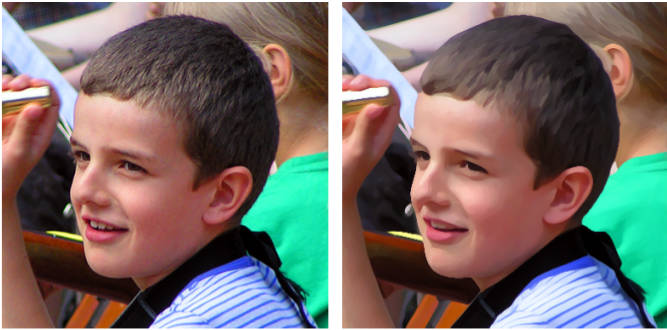
\includegraphics[width=0.7\textwidth]{filterskid}
    \caption{Comparação entre imagem não abstraída (esquerda) e imagem abstraída (direita) \cite{Kyprianidis2009}.}	
    \label{fig:filterskid}
  \end{center}
\end{figure}

Ao nível dos filtros de abstração o estudo será efetuado utilizado o filtro Kuwahara Anisotrópico (FKA).

Este filtro consiste numa generalização do filtro Kuwahara (ver \ref{subsec:kuwahara}) que remove alguns artefactos originados na aplicação do filtro original através da adaptação da forma, escala e orientação do filtro à estrutura local das características da imagem \cite{Kyprianidis2009}. Desta forma é produzido um efeito de abstração tipo pintura, onde é removida informação não essencial em zonas de elevado contraste, enquanto são preservados os limites representados nas zonas de menor contraste, tal como demonstrado na figura \ref{fig:filterskid}. As imagens ficam assim com a clareza de uma ilustração, mas preservam a informação direcional tal como nas pinturas a óleo clássicas. Por outro lado, este filtro tira partido da placa gráfica para a realização da abstração das imagens, tornando-se assim particularmente indicado para o processamento de um elevado número de fotografias.

O filtro em questão foi também utilizado anteriormente, e com resultados positivos, em abstração de imagens para a recuperação de informação multimédia. 

Tendo em conta os fatores apresentados consideramos que este filtro é o mais adequado para a utilização no âmbito deste projeto.

\section{Coleções de dados}
Ao nível das coleções de dados a analisar, temos em vista a utilização de duas coleções a primeira é a uma coleção standard, chamada \textit{Labeled Faces in the Wild} e que permite obter resultados comparativos com avaliações efetuadas anteriormente a sistemas de reconhecimento facial existentes. A segunda é a coleção de imagens Sapo Fama, qual agrega uma base de dados de imagens de personalidades famosas nacionais e internacionais, representado uma possível área de aplicação do sistema desenvolvido.

\subsection{\textit{Labeled Faces in the Wild}}
A coleção \textit{Labeled Faces in the Wild (LFW)} é uma base de dados fotográfica desenhada especificamente para o estudo do problema de reconhecimento facial, particularmente em situações onde as condições de captura das imagens não possuem restrições. Esta coleção possuí 13233 imagens, de 5749 pessoas diferentes, sendo que dessas pessoas 1680 possuem mais do que uma imagem na galeria. O uso desta galeria no âmbito desta dissertação permitirá efetuar uma análise dos resultados obtidos num conjunto de dados standard e já previamente analisado por outros investigadores, assim como agilizar os testes dos sistemas desenvolvidos uma vez que a coleção já se encontra preparada especificamente para o estudo do desempenho de sistemas de reconhecimento facial automático. Nas figuras \ref{fig:galeria}, \ref{fig:gp} e \ref{fig:gn} encontram-se representados alguns exemplos das imagens contidas nesta coleção e respetivas anotações.

\subsection{Sapo Fama}
\begin{figure}[ht]
  \begin{center}
    \leavevmode
    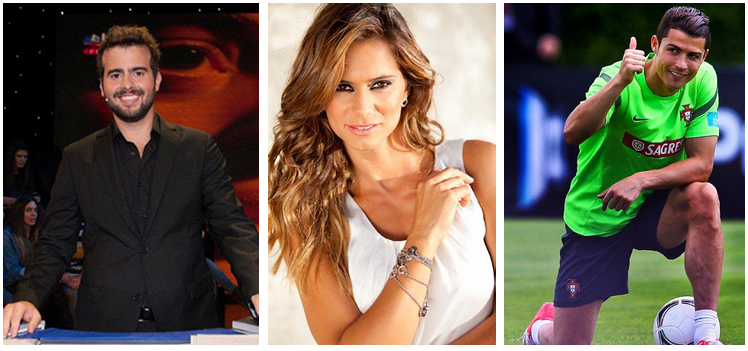
\includegraphics[width=0.9\textwidth]{sapoFama.png}
    \caption{Exemplos de imagens da coleção Sapo Fama \cite{PTC2011}.}	
    \label{fig:sapoFama}
  \end{center}
\end{figure}
A coleção Sapo Fama irá ser disponibilizada no âmbito da integração desta dissertação no laboratório de investigação da Sapo da Universidade do Porto. Esta galeria multimédia agrega uma coleção de imagens utilizadas na plataforma online de notícias sobre personalidades públicas da Sapo, capturadas num grande número de eventos com condições de iluminação, pose e expressão facial muito variáveis. Para além disso, a cada imagem encontra-se ainda associada uma descrição textual. As imagens contidas nesta coleção representam uma oportunidade única de avaliação do sistema desenvolvido numa biblioteca de imagens real e com elevado valor comercial. Na figura \ref{fig:sapoFama} encontram-se representados alguns exemplos das imagens contidas nesta coleção.

Para a utilização deste conjunto de dados será ainda necessário efetuar a preparação do mesmo nomeadamente através da extração e segmentação das diversas entidades presentes em cada imagem, assim como da normalização das imagens, por exemplo, em termos de dimensão.

\section{Avaliação Desempenho}
A avaliação da desempenho dos sistemas de reconhecimento facial é normalmente efetuada em duas situações específicas: identificação e verificação de faces. No âmbito da avaliação desses sistemas designam-se de $amostras$ $biometricas$ as capturas de características de uma pessoa que permitem efetuar o seu reconhecimento. Dependendo do sistema essas amostras podem ser apenas uma imagem, um conjunto de imagens ou até um vídeo. Designa-se ainda de $prova$ a amostra biométrica apresentada ao sistema para ser reconhecida.

Para uma avaliação precisa dos sistemas automáticos de reconhecimento facial são necessários três conjuntos de imagens:
\begin{figure}[ht]
  \begin{center}
    \leavevmode
    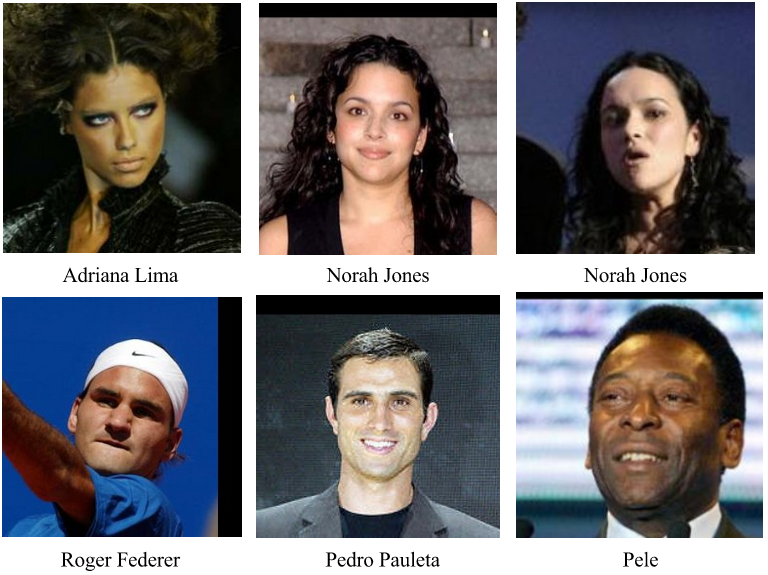
\includegraphics[width=0.9\textwidth]{galeria.png}
    \caption{Galeria com faces conhecidas pelo sistema e respectivas anotações \cite{UniversityofMassachussets}.}	
    \label{fig:galeria}
  \end{center}
\end{figure}
O primeiro, conjunto $\mathscr{G}$, designado de galeria, contem amostras biométricas das pessoas já conhecidas pelo sistema. Um exemplo de imagens da galeria pode ser visto na figura \ref{fig:galeria}

\begin{figure}[ht]
  \begin{center}
    \leavevmode
    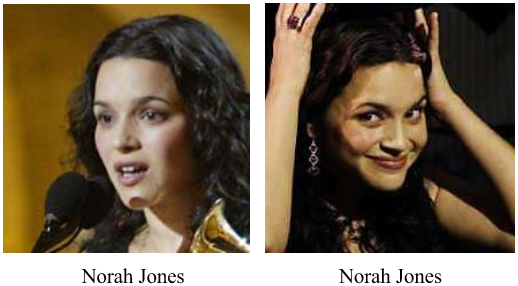
\includegraphics[width=0.6\textwidth]{gp.png}
    \caption{Imagens de pessoas conhecidas pelo sistema, mas não presentes na galeria \cite{UniversityofMassachussets}.}	
    \label{fig:gp}
  \end{center}
\end{figure}
O segundo grupo de imagens é o conjunto $\mathscr{P}_\mathscr{G}$ e engloba o conjunto de provas de pessoas conhecidas pelo sistema, mas que são diferentes das amostras biométricas presentes na galeria. Um exemplo de imagens deste conjunto pode ser visto na figura \ref{fig:gp}, onde se encontram representadas imagens da cantora Norah Jones, mas que são diferentes das imagens presentes no conjunto $\mathscr{G}$.

\begin{figure}[ht]
  \begin{center}
    \leavevmode
    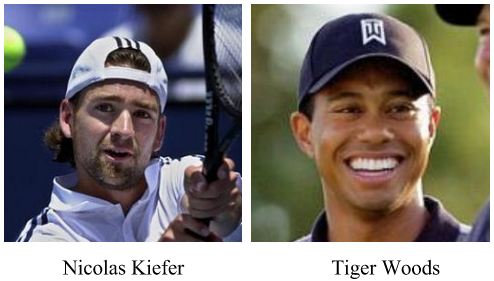
\includegraphics[width=0.6\textwidth]{gn.png}
    \caption{Imagens de pessoas não conhecidas pelo sistema \cite{UniversityofMassachussets}.}	
    \label{fig:gn}
  \end{center}
\end{figure}
O último conjunto é designado de $\mathscr{P}_\mathscr{N}$, e corresponde ao conjunto de provas de pessoas não presentes na galeria. Essas imagens são também muitas vezes designadas de impostores, uma vez que servem para testar as situações em que o sistema identifica erradamente pessoas desconhecidas pelo sistema como pessoas presentes na galeria. Um exemplo deste conjunto de imagens encontra-se representado na figura \ref{fig:gn}

Quando uma prova $p_j$ é apresentada ao sistema, essa prova é então comparada a cada amostra biométrica $g_i$ da galeria, resultando dessa comparação o respetivo índice de similaridade (\textit{similarity score}), $s_{ij}$. Este índice é designado de $match$ $score$, caso $g_i$ e $p_j$ sejam amostras da mesma pessoa, caso não o sejam é designado de $nonmatch$ $score$.

A função $id()$ retorna a identidade de uma amostra biométrica, em que $id(p_j) = id(g^*)$, sendo $g^*$ a única correspondência de $p_j$ na galeria e $s_{*j}$ o respetivo índice de similaridade.

De seguida, encontra-se descrita brevemente a forma como é efetuada a avaliação da desempenho dos sistemas de reconhecimento facial para os casos de identificação e verificação.

\subsection{Identificação}
Tal como referido no capítulo \ref{chap:reco} deste relatório, em sistemas de reconhecimento facial automático o problema de identificação consiste na determinação da identidade de uma amostra biométrica (prova) fornecida ao sistema.

Na identificação de uma dada prova são calculados os índices de similaridade para todas as amostras na galeria, e ordenados os seus resultados. Uma prova $p_j$ tem ranking $n$ se o seu índice de similaridade for o enésimo maior índice de similaridade. Caso haja empates nos índices de similaridade é necessário resolver esses empates para determinar o ranking de uma prova, havendo para isso três métodos: otimista, pessimista e média. No método otimista, uma prova é associada ao ranking mais alto possível, obtido pelo número de índices estritamente maiores do que $s_{*j}$ mais um ($|> s_{*j}| + 1$). Na abordagem pessimista, um prova é associada ao ranking mais baixo possível, sendo esse devolvido pelo número de índices maiores ou iguais a $s_{*j}$ mais um ($|\geqslant s_{*j}| + 1$). Na média, tal como o seu nome indica é efetuada uma média entre os valores obtidos pelos métodos pessimista e otimista, sendo esta a abordagem mais utilizada. 

O desempenho da identificação em sistemas de reconhecimento facial pode ser avaliada em taxa de deteção e identificação e taxa de falso-alarme:

 \begin{description}
 \item[Taxa de deteção e identificação $(T_{DI})$:] Percentagem de provas do conjunto $\mathscr{P}_\mathscr{G}$ que são corretamente  identificadas. Uma prova é corretamente identificada caso o índice de similaridade para o seu $match$ $score$ seja seja maior do que um limite operacional pré-definido $\tau$.
\begin{equation}
 T_{DI}(\tau, n) = \frac{|\{p_j:p_j \in \mathscr{P}_\mathscr{G}, rank(p_j) \leqslant n, s_{*j} \geqslant \tau\}|}{|\mathscr{P}_\mathscr{G}|}
\end{equation}
 Em que no caso de se pretender apenas determinar a identificação da pessoa é devolvido apenas o \textit{top match}, ou seja o resultado com ranking $n=1$. Caso contrário, podem ser devolvidos todos os primeiros $n$ resultados com índice de similaridade superior ao limite operacional estabelecido.
 
  \item[Taxa de falso-alarme $(T_{FA})$:] Percentagem de impostores identificados erradamente, ou seja, percentagem de pessoas do conjunto de provas $\mathscr{P}_\mathscr{N}$, identificadas como alguém presente na galeria $\mathscr{G}$.  
\begin{equation}
 T_{FA}(\tau) = \frac{|\{p_j:p_j \in \mathscr{P}_\mathscr{N}, s_{ij} \geqslant \tau\}|}{|\mathscr{P}_\mathscr{N}|}
\end{equation}
\end{description}

Um sistema de reconhecimento facial ideal teria uma taxa de deteção e identificação de 1.0 e uma taxa de falso-alarme de 0.0.

\subsection{Verificação}
Em situações de verificação da identidade, para além de uma amostra biométrica ($prova$) é também fornecida ao sistema a identidade da pessoa que se pretende identificar. Cabe ao sistema determinar se a identidade e amostra fornecidas pertencem à mesma pessoa. O sistema compara então a prova à amostra biométrica guardada na galeria, da pessoa a quem corresponde a identidade fornecida. Da comparação efetuada resulta o índice de similaridade entre a prova fornecida e os dados já armazenados no sistema.

Em termos formais, a verificação pode ser avaliada pela taxa de verificação e taxa de falso-alarme, as quais podem ser descritas da seguinte forma:

\begin{description}
 \item[Taxa verificação $(T_{V})$:] Percentagem de provas do conjunto $\mathscr{P}_\mathscr{G}$ que são corretamente verificadas. O sistema aceita como verdadeira a identidade fornecida caso o índice de similaridade calculado seja superior a um  limite operacional fornecido.

\begin{equation}
 T_{V}(\tau, n) = \frac{|\{p_j:p_j \in \mathscr{P}_\mathscr{G}, s_{ij} \geqslant \tau, id(g_i)=id(p_j)\}|}{|\mathscr{P}_\mathscr{G}|}
\end{equation}

  \item[Taxa de falsa-aceitação $(T_{FA})$:] Percentagem de impostores aceites erradamente, ou seja, percentagem de pessoas do conjunto de provas $\mathscr{P}_\mathscr{N}$, verificadas como alguém presente na galeria $\mathscr{G}$.
  
\begin{equation}
 T_{FA}(\tau) = \frac{|\{p_j:p_j \in \mathscr{P}_\mathscr{N}, s_{ij} \geqslant \tau\}|}{|\mathscr{P}_\mathscr{N}||\mathscr{G}|}
\end{equation}
\end{description}

\begin{figure}[ht]
  \begin{center}
    \leavevmode
    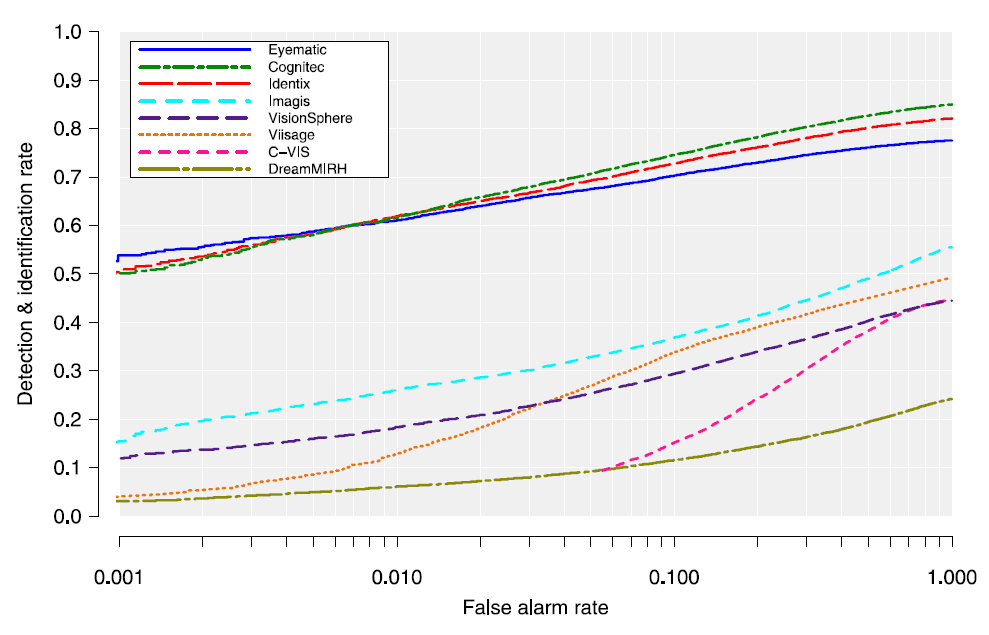
\includegraphics[width=0.8\textwidth]{roc.png}
    \caption{ROC computado durante os FRVT 2002 \cite{Li2011}.}	
    \label{fig:roc}
  \end{center}
\end{figure}
A modificação do valor de $\tau$ tem influência direta nas percentagens de deteção e/ou verificação e de falsos-alarmes calculadas. Ao aumentar o limite operacional, ambas as taxas diminuem, não sendo por isso possível maximizar ambos os valores, uma vez que existe sempre um compromisso entre o aumento da taxa de deteção e identificação e o aumento do número de falsos-alarmes. Este compromisso é tradicionalmente representado num gráfico do tipo \textit{receiver operating characteristic} (ROC). Um exemplo de um ROC encontra-se representado na figura \ref{fig:roc}, com um ranking constante de 1. 

\begin{figure}[ht]
  \begin{center}
    \leavevmode
    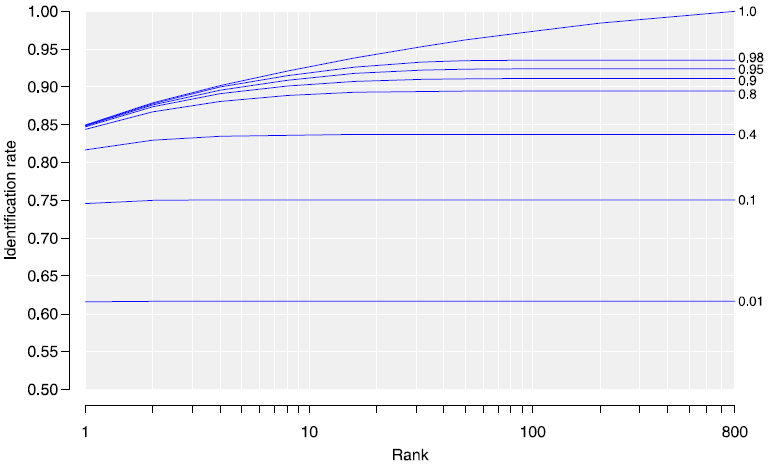
\includegraphics[width=0.8\textwidth]{roc2.png}
    \caption{Desempenho em identificação para 8 níveis de taxas de falso-alarme. A curva superior corresponde a uma taxa de falso alarme de 1.0 \cite{Li2011}.}	
    \label{fig:roc2}
  \end{center}
\end{figure}
Outra forma de representar a performance de sistemas de reconhecimento facial é em função do ranking das provas presentes na galeria e encontra-se representada na figura \ref{fig:roc2}. Nesta figura, o eixo vertical representa a taxa de deteção e reconhecimento e o eixo horizontal o ranking numa escala logarítmica. Cada curva representa a performance do mesmo sistema com uma diferente taxa de falso-alarme.

\section{Resultados Esperados}
Tendo em conta os resultados anteriormente observados no recurso à utilização de filtros de abstração para a ilustração automática de texto e o estado da arte da área de reconhecimento facial automático em imagens, esperamos, no contexto desta dissertação, determinar o impacto do uso da abstração de imagens no processo de reconhecimento facial automático, nomeadamente nos seguintes pontos:
\begin{itemize}
\item Eficácia do reconhecimento;
\item Necessidades de processamento das imagens;
\item Necessidades de armazenamento das imagens.
\end{itemize}
Para além do impacto ao nível do desempenho com o uso de abstração de imagens, esperamos determinar qual o compromisso existente entre a eficácia do reconhecimento e as necessidades de processamento e armazenamento das imagens.

\section{Plano de Trabalho}
Na figura \ref{fig:gantt} encontra-se representado o plano de trabalho para a disciplina de dissertação. Este plano engloba um período de 25 semanas, com início na segunda semana do mês de Fevereiro e fim na última semana do mês de Julho, sendo que as últimas quatro semanas do mês de Julho se encontram reservadas para o período de realização das provas públicas de dissertação.

\begin{figure}[ht]
	\begin{center}
		\begin{gantt}[xunitlength=0.4cm,fontsize=\small,titlefontsize=\small,drawledgerline=true]{10}{25}
		\begin{ganttitle}
		 \titleelement{Feb}{3}
		 \titleelement{Mar}{4}
		 \titleelement{Apr}{5}
		 \titleelement{May}{4}
		 \titleelement{Jun}{4}	
		 \titleelement{Jul}{5}
		\end{ganttitle}
		\begin{ganttitle}
		 \titleelement{2}{1}
		 \titleelement{3}{1}
		 \titleelement{4}{1}
		 \titleelement{1}{1}
		 \titleelement{2}{1}
		 \titleelement{3}{1}
		 \titleelement{4}{1}
		 \titleelement{1}{1}
		 \titleelement{2}{1}
		 \titleelement{3}{1}
		 \titleelement{4}{1}
		 \titleelement{5}{1}
		 \titleelement{1}{1}
		 \titleelement{2}{1}
		 \titleelement{3}{1}
		 \titleelement{4}{1}
		 \titleelement{1}{1}
		 \titleelement{2}{1}
		 \titleelement{3}{1}
		 \titleelement{4}{1}
		 \titleelement{1}{1}
		 \titleelement{2}{1}
		 \titleelement{3}{1}
		 \titleelement{4}{1}
		 \titleelement{5}{1}
		\end{ganttitle}
		\ganttbar{1. Sistema Reconhecimento Facial Base}{0}{4}
		\ganttbar{2. Experiências Conjunto Dados}{2}{2}
		\ganttbar{3. Preparação Conjunto Dados}{3}{4}
		\ganttbar{4. Avaliação Desempenho sem Filtros}{5}{4}
		\ganttbar{5. Aplicação Filtros e Adaptação Sistema}{8}{4}
		\ganttbar{6. Análise Impacto Filtros Abstração}{9}{7}
		\ganttbar{7. Escrita Dissertação}{7}{14}
		\ganttbar{8. Escrita Artigo}{16}{5}
		\end{gantt}
		\caption{Plano Trabalho 2º Semestre.}
		\label{fig:gantt}
	\end{center}
\end{figure}

O plano de trabalho engloba um conjunto de oito tarefas. A primeira tarefa consiste na implementação de um sistema de reconhecimento facial base com recurso à biblioteca OpenCV. Paralelamente, irão também ser realizadas algumas experiências com os conjuntos de dados a utilizar de forma a determinar as necessidades de preparação e adaptação dos dados existentes.

A terceira e quarta tarefas compreendem a preparação do conjunto de dados de acordo com as necessidades determinadas na tarefa anterior e a posterior avaliação do desempenho do sistema criado sem a utilização de filtros de abstração.

A quinta e sexta tarefa dizem respeito à aplicação dos filtros de abstração às coleções de dados existentes e a posterior adaptação e avaliação do sistema de reconhecimento facial anteriormente desenvolvido com a utilização de imagens abstraídas.

Finalmente, as últimas duas tarefas englobam a escrita da dissertação e a escrita de um artigo científico acerca dos resultados obtidos.
%Adicionalmente propõe-se também o desenvolvimento de um sistema de reconhecimento facial de personalidades que integre a abstração de imagens no processo de reconhecimento facial. Este sistema deverá ser capaz de detetar as faces presentes numa imagem e apresentar uma lista de possíveis entidades nela contidas.
